% !TeX root = ../diss.tex

\chapter{Preparation}

There were two main areas of preparation for my project. One was to research the Smith-Waterman (SW) algorithm, and the ways it has been modified and implemented by others.
The other area was researching the different architectures, programming environment and tools to use.

\section{Overview of the Smith-Waterman algorithm}
\label{sec:SW_Overview}
Sequence alignment algorithms are used to find similar regions between two strings.
This involves predicting where symbols in the two strings correlate with each other (both matching and mismatching symbols), or where one sequence has some symbols that have been inserted into that sequence or deleted from the other.
This can be represented as follows, where symbols in the same column correspond to one another, and dashes represent insertions or deletions (gaps):
\begin{center}
\begin{tabular}{c}
\begin{lstlisting}[basicstyle=\ttfamily\linespread{0.8}]
AC-T
ACGT
\end{lstlisting}
\end{tabular}
\end{center}

The Smith-Waterman algorithm \cite{SW_Original} is a local alignment algorithm; it can produce alignments that span a subset of the input sequences.
This is useful when aligning long segments of DNA which contain non-coding regions or multiple different genes (which occurs when aligning against an entire chromosome).
When aligning a single gene against a chromosome from a different species, a local alignment algorithm can find the relevant region whilst excluding the rest of the longer sequence in the alignment.

\subsection{The Dynamic Programming approach}
\label{sec:SW_DP}

The Smith-Waterman algorithm \cite{SW_Original} finds alignments using dynamic programming.
For sequences $A=a_1 a_2 \ldots a_N$ and $B=b_1 b_2 \ldots b_M$, a scoring matrix $H$ is constructed where cell $H_{i,j}$ gives the score of the best local alignment that ends with $a_i$ and $b_j$.
Using a similarity function $s(a,b)$ which gives the similarity of two sequence symbols, and gap score list $W_k$ which gives the penalty for a deletion of length $k$, $H_{i,j}$ is defined as follows:
$$ H_{i,j} = \max \begin{cases}
H_{i-1,j-1} + s(a_i, b_j) & \text{(Including both symbols in alignment)} \\
\max_{k \geq 1}(H_{i-k,j} - W_k) & \text{(Skipping $k$ symbols from $a$)} \\
\max_{l \geq 1}(H_{i,j-l} - W_l) & \text{(Skipping $k$ symbols from $b$)} \\
0 & \text{(Starting alignment here)}
\end{cases}$$

The grid is initialised using $\forall i\leq N . H_{i,0}=0$ and $\forall j \leq M . H_{0,j}=0$.

For example, using sequences {\ttfamily GACT} and {\ttfamily ACGT} and the following definitions of $s(a,b)$ and $W_k$:
$$s(a, b)= \begin{cases}
5 &  a = b \\
-4 & a \neq b
\end{cases}
\qquad \qquad \qquad W_k = -k
$$

\begin{center}
$H = $ \begin{tabular}{|c|ccccc|} \hline
& & {\ttfamily A} & {\ttfamily C} & {\ttfamily G} & {\ttfamily T} \\ \hline
& $0$ & $0$ & $0$ & $0$ & $0$ \\
{\ttfamily G} & $0$ & $0$ & $0$ & $3$ & $2$ \\
{\ttfamily A} & $0$ & $3$ & $2$ & $2$ & ${\color{darkorange} 1}$ \\
{\ttfamily C} & $0$ & $2$ & ${\color{darkblue}6}$ & $5$ & $4$ \\
{\ttfamily T} & $0$ & $1$ & $5$ & $4$ & $8$ \\ \hline
\end{tabular}
\end{center}

Taking two examples from this:
\begin{align*}
{\color{darkblue}H_{3,2}} = 6 &= \max \begin{cases}
    3 + s(\text{\ttfamily C}, \text{\ttfamily C}) =6\\
    \max(2-1, 0 - 2, 0-3) =1 \\
    \max(2-1, 0 - 2) =1\\
    0
\end{cases} \\
{\color{darkorange} H_{2,4}} = 1 &= \max \begin{cases}
    3 + s(\text{\ttfamily A}, \text{\ttfamily T}) =1 \\
    \max(2-1, 0 - 2) =1 \\
    \max(2-1, 2 - 2, 3-3, 0-4) =1 \\
    0
\end{cases}
\end{align*}
Note that in the case of $H_{2,4}$ (and others) there are multiple ways of getting to the maximum value (from above, the left, or diagonally in this case), and this leads to multiple alignments that have the same optimal score.

\subsection{Back-tracing}
\label{sec:SW_Back_tracing}
Stored with each grid cell is a ``pointer'' which locates the previous cell in the alignment ending with that cell, where pointer $p \in \{Above_k, Left_k, Diagonal, Nil\}$. $Nil$ represents this cell not being part of an alignment, because all paths to that cell are worse than the threshold $0$. $Left_k$ represents skipping $k$ symbols from $a$, likewise for $Above_k$ skipping $k$ symbols from $b$. In the general case, this matrix of pointers $P$ is found using:
$$ P_{i,j} = \begin{cases}
    Diagonal, & H_{i,j} = H_{i-1,j-1} + s(a_i, b_j) \\
    Left_k, & H_{i,j} = \max_{k \geq 1}(H_{i-k,j} - W_k) \\
    Above_k, & H_{i,j} = \max_{l \geq 1}(H_{i,j-l} - W_l) \\
    Nil, & H_{i,j} = 0
\end{cases}$$
\pagebreak

An example of $P_{i,j}$ is as follows (where $\cdot$ represents $Nil$):
\begin{center}
$P = $     \begin{tabular}{|p{0.035\textwidth}|p{0.035\textwidth}p{0.035\textwidth}p{0.035\textwidth}p{0.035\textwidth}p{0.035\textwidth}|} \hline
& & \hfil {\ttfamily A} & \hfil {\ttfamily C} & \hfil {\ttfamily G} & \hfil {\ttfamily T} \\ \hline
& \hfil $\cdot$ & \hfil $\cdot$ & \hfil $\cdot$ & \hfil $\cdot$ & \hfil $\cdot$ \\
\hfil {\ttfamily G} & \hfil ${\color{darkorange} \cdot}$ & \hfil $\cdot$ & \hfil $\cdot$ & \hfil $\nwarrow$ & \hfil $\leftarrow_1$ \\
\hfil {\ttfamily A} & \hfil $\cdot$ & \hfil ${\color{darkorange} \nwarrow}$ & \hfil $\leftarrow_1$ & \hfil $\uparrow_1$ & $\leftarrow_1$ \\
\hfil {\ttfamily C} & \hfil $\cdot$ & \hfil $\uparrow_1$ & \hfil ${\color{darkorange} \nwarrow}$ & \hfil ${\color{darkorange} \leftarrow_1}$ & $\leftarrow_2$ \\
\hfil {\ttfamily T} & \hfil $\cdot$ & \hfil $\uparrow_2$ & \hfil $\nwarrow$ & \hfil $\leftarrow_1$ & \hfil ${\color{darkorange} \nwarrow}$ \\ \hline
\end{tabular}
\end{center}

A running maximum score is maintained during the production of the grid, and the cell $H_{i,j}$ with the highest score corresponds to the highest-scoring alignment, which finishes with $a_i$ and $b_j$.
Starting here, the alignment can be found from end to start by following the pointers in the grid. The best path through $P_{i,j}$ is highlighted in {\color{darkorange}orange}, and gives alignment:
\begin{center}
\begin{tabular}{c}
\begin{lstlisting}[basicstyle=\ttfamily\linespread{0.8}]
AC-T
ACGT
\end{lstlisting}
\end{tabular}
\end{center}

\subsection{Algorithmic complexity}
\label{sec:SW_Complexity}
For sequences of lengths $N$ and $M$, this algorithm requires $O(NM)$ space to store the two matrices, each with $(N+1)\times(M+1)$ elements.
The runtime is $O(N^2 M)$, where without loss of generality $N\geq M$.
Each cell needs to consider the cell to its diagonal (constant time), and all of the cells above it (of order $M$ cells), and all cells to its left (of order $N$ cells).
This gives a runtime for evaluating a cell as $O(N+M)$, which is $O(N)$ given $N\geq M$.
There are $NM$ cells to be evaluated, so producing the grid takes $O(N^2 M)$ time.

If the gap evaluation scheme did not maximise over a row, and instead performed constant time operations, then the complexity is $O(NM)$.
This is discussed in \cref{sec:SW_gaps}.

Each back-tracing step requires constant time (a matrix lookup, and some pointer comparisons) to produce each element in the alignment, and the length of alignment is bounded by $N+M$, where the alignment is wholly made up of gaps.
Therefore, this step requires $O(N)$ space and time, where $N\geq M$.

Overall, the space requirements of the algorithm as presented is $O(NM)$, and the time requirements are either $O(NM)$ or $O(N^2 M)$ depending on how gaps are evaluated.
Improvements to this are discussed in \cref{sec:SW_Linear_Prep}.

\subsection{Scoring alignments}
\label{sec:SW_Scoring}

The general approach to scoring alignments is given in the paper written by Smith and Waterman \cite{SW_Original}, but the exact details are not specified.
There are two areas that need definition: how to compare a pair of sequence symbols, and how to score gaps in the alignment.

\subsubsection{Sequence similarity functions}
\label{sec:SW_similarity_functions}
The original paper requires similarity function $s(a,b)$ which gives the similarity of two sequence symbols. One simple implementation might be:
$$s(a, b) = \begin{cases}
m,   & a =    b \\
\mu, & a \neq b
\end{cases}$$

For two constants $m$ and $\mu$ where typically $m>0$ and $\mu<0$.
The implementation Smith-Waterman in the European Molecular Biology Open Software Suite (EMBOSS) \cite{EMBOSS} uses an approach equivalent to using $m=5$ and $\mu=-4$ for DNA alignments by default.

However, the biological processes that leads to one symbol being substituted for another cannot be entirely expressed in these two constants, especially when some symbols are more likely than others to replace a given symbol.
This is particularly problematic in proteins, which naturally are made up of 22 different types of amino acids.

A more granular approach is to base $s(a,b)$ on a substitution matrix, which encodes a score for each different pairing of symbols.
This has performance penalties (\cref{sec:C_scoring_eval,sec:CUDA_scoring_eval,sec:SV_expected_v_actual,sec:FPGA_utilisation,sec:SV_Fmax}), because the first approach can use direct equality testing and hard-coded constants, whereas using a substitution matrix for proteins requires a lookup from a $22\times22$ matrix.

Discussions of which substitution matrices are best for which applications are beyond the scope of this project, and they are all implemented in the same way.
I chose to base investigations into the performance implications into this on the BLOSUM50 matrix for proteins \cite{BLOSUM}, which is used for alignments between sequences that are not closely related.

\subsubsection{Scoring gaps}
\label{sec:SW_gaps}
The original paper \cite{SW_Original} references a gap weight vector $W_k$, which defines the score penalty of a gap of length $k$, where gaps jump either $k$ elements to the left, or above.
However, it makes the algorithm run in $O(N^2 M)$ time for $N\geq M$ (\cref{sec:SW_Complexity}), so other approaches are used instead.

One solution to this problem was suggested by Waterman and Smith \cite{SW_Metrics} in an earlier paper about global alignment: to define $W_k=kw_1$ for some gap penalty $w_1$.
Using the recursive definition of $H_{i,j}$ the score using a $Left$ gap is:
$$\max_{k \geq 1}(H_{i-k,j} -W_k) = H_{i-1,j} - w_1$$
Gotoh proposed a different way of solving this problem \cite{Gotoh}.
The constant gap penalty models the cost of inserting or deleting symbols in a sequence by making this penalty proportional to the length of the insertion or deletion.
This is not ideal, because as Gotoh observes, ``long gap[s] can be produced by a single mutational event''.
Instead he proposes what is later called the affine-gap method, where $W_k=uk+v$ for some gap penalties $u$ and $v$.
The penalty of starting to insert or delete a sequence is given by $u$, and $v$ accounts for the different lengths of such a sequence.

This approach requires more space than the original Smith-Waterman algorithm because choosing whether to open a gap has an impact on scores later in the alignment.
When evaluating a mismatched cell in the dynamic-programming grid it is impossible to know whether to pay the mismatch penalty because a sequence of matches immediately follow, or if a long sequence of mismatches follow and it would be less expensive to open up a gap to cover them instead.
Therefore, extra space is needed to keep track of scores when the decision to open a gap is and also is not taken.

To achieve this, three grids are constructed instead of one.
This triples the memory requirements in practice but does not change the asymptotic memory requirements.
The main score grid $H_{i,j}$ is calculated using a similar approach to before, representing the score of the best alignment using sequences $a_1\ldots a_i$ and $b_1 \ldots b_j$.
Additionally, there is grid $F_{i,j}$ which represents the score of the best alignment between $a_1\ldots a_i$ and $b_1 \ldots b_j$ provided it ended with an open left-gap.
$G_{i,j}$ is similar for above gaps.
This gives grid definitions:
\begin{align*}
H_{i,j} &= \max(H_{i-1,j-1} + s(a_i, b_j), F_{i,j}, G_{i,j}, 0) \\
F_{i,j} &= \max(H_{i-1,j} + u + v, F_{i-1,j} + v) \\
G_{i,j} &= \max(H_{i,j-1} + u + v, G_{i,j-1} + v)
\end{align*}

This is modified from the original paper somewhat for notational consistency with the rest of the dissertation.

Pointer grids need to be stored for all three grids, where the back-tracer will start in grid $H$ (and this is the only grid where the running maximum is kept), but it will trace through $F$ and $G$ as well to determine where a gap started.

\subsection{Linear space modification to Smith-Waterman algorithm}
\label{sec:SW_Linear_Prep}
\subsubsection{Overview}
\label{sec:SW_Linear_Overview}

A common approach to improving the runtime of the Smith-Waterman algorithm is to reduce the amount of space used by increasing the amount of time spent in doing arithmetic.
Hirschberg’s algorithm \cite{Hirschberg} pioneered this approach for the Longest Common Subsequence problem.
Myers and Miller apply this approach to local alignments \cite{MyersMiller}, which is summarised below.

The purpose of this algorithm is to correctly and efficiently split the alignment into small chunks, manageable for the quadratic space implementation which is where the back-tracing is done.
It recursively divides a large grid into two smaller grids.
\Cref{fig:Linear_Space_Structure} shows this, where the optimal alignment is shown in orange.
The grid has been divided into two smaller grids by the first pass of the algorithm, a grid with blocks $1$ and $2$, and the grid with blocks $3$ and $4$.
The grey segments do not contain the alignment and can be ignored.
The black arrows represent the direction the blocks are evaluated in, discussed further on.

\Cref{lst:pseudo_sw} is a pseudo-code representation of the quadratic space Smith-Waterman algorithm, to be used in this linear space algorithm.
Parameter \lstinline{fixedTop} specifies whether the alignment can start from anywhere in the grid, or just the top left corner (and is implemented by including or removing the options of $0$ and $Nil$ from the maximising functions).
This is necessary because the optimal alignment inside a subproblem may not start at the top-left, but the overall optimal alignment may pass through multiple sub-grids where the top-left of each grid must be connected to the bottom-right of the next grid.
Parameter \lstinline{fixedBottom} is similar, specifying whether to start back-tracing at the best cell in the grid, or the bottom-right cell.

\begin{figure}
    \centering
    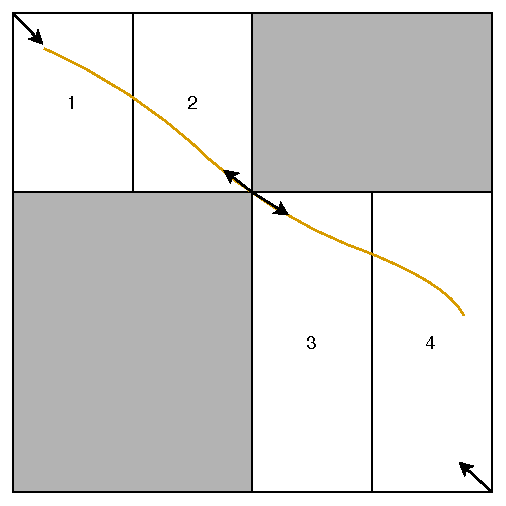
\includegraphics[width=(0.4\textwidth)]{figs/linear_space_structure.pdf}
    \caption{The divided dynamic programming matrix when using the linear space approach, after the first iteration}
    \label{fig:Linear_Space_Structure}
\end{figure}

\begin{lstlisting}[basicstyle=\linespread{0.9}\ttfamily\footnotesize, label={lst:pseudo_sw},captionpos=b,caption={Pseudo-code representation of quadratic space implementation of SW algorithm}]
fun sw(seq1, seq2, fixedTop, fixedBottom):
    Dynamic programming approach using quadratic space
    if fixedTop:
        Only allow alignments to start at the top-left
    else:
        Allow alignments to start anywhere
    if fixedBottom:
        Return the alignment ending at the bottom-right grid cell
    else:
        Return the alignment ending at the best cell in the grid
\end{lstlisting}

To split a large grid into two smaller grids, the scores of the middle column of cells are found by starting from the top-left and working towards the middle, and also by starting from the bottom right and working towards the middle.
\Cref{lst:pseudo_sw_col} is a representation of this.
In \cref{fig:Linear_Space_Structure}, blocks $1$ and $3$ are evaluated from their top-lefts to their middle columns, and blocks $2$ and $4$ from the bottom-right, and the direction of evaluation represented by the black arrows.
These scores are found using a linear space.
These two columns are added together, and each cell of the column gives the score for the best alignment that passes through that cell.
The optimal alignment might cross the middle column or be in one of these half-grids.

The middle columns are found using $O(N)$ space for sequences of lengths $N$ and $M$, and maintains $O(NM)$ time complexity, albeit with a greater constant factor.
This uses the fact that only the immediate neighbours are needed to calculate the score of a cell, so the values of a previous column can be discarded once the values in the next column have been computed. This data dependency is shown in \cref{fig:Linear_Space_Dependencies}.
However, discarding this information leads to recomputation of the cells in the smaller subproblems that are recursively evaluated.

Maxima are calculated whilst computing each half, and compared to the maximum cell in the summed columns.
If the overall maximum is in one of the half-grids, restart the algorithm between that cell and the top-left or bottom-right, if on the left or right sides respectively.
Otherwise, the algorithm is rerun between the end cells and the maximum middle cell.
This recursively breaks up the alignment until it is small enough to tackle directly using the quadratic space algorithm (\cref{sec:SW_DP,sec:SW_Back_tracing,sec:SW_Complexity}), and then joins them back together.
\begin{figure}[h]
    \centering
    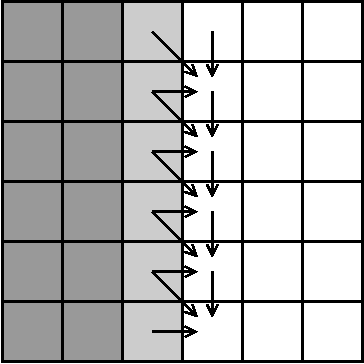
\includegraphics[width=(0.4\textwidth)]{figs/linear_space_deps.pdf}
    \caption{Data dependencies when using the linear space approach}
    \label{fig:Linear_Space_Dependencies}
\end{figure}
\begin{lstlisting}[basicstyle=\ttfamily\linespread{0.9}\footnotesize, label={lst:pseudo_sw_col},captionpos=b,caption={Pseudo-code representation of linear space algorithm which finds middle columns}]
    fun sw_col(seq1, seq2, direction, fixedStart):
        direction in {forwards, backwards}
        direction determines which half of grid is evaluated
            - Forwards: from top left, to column (seq2/2)
            - Backwards: from bottom right, to column (seq2/2)
        fixedStart similar to fixedTop of sw()
        Calculate grid column by column, returning:
            - Values of column (seq2/2)
            - Location of best cell, and score
    \end{lstlisting}
\begin{minipage}{\linewidth}
\begin{lstlisting}[basicstyle=\linespread{0.9}\ttfamily\footnotesize, label={lst:pseudo_sw_linear},captionpos=b,caption={Pseudo-code representation of the linear space Smith-Waterman algorithm}]
fun sw_linear(seq1, seq2, fixedTop, fixedBottom):
    if seq1 and seq2 are small:
        return sw(seq1, seq2, fixedTop, fixedBottom)
    else:
        (forwardCol, bestForwards) = sw_col(seq1, seq2, forwards, fixedTop)
        (backwardCol, bestBackwards) = sw_col(seq1, seq2,
                                              backwards, fixedBottom)
        middleCol = forwardCol + backwardCol # Using vector addition
        bestMiddle = max(middleCol)

        # Using list splicing: seq1[x:] = [seq1[x], seq1[x+1], ... seq1[n]]
        if best path is bottom-right to bestBackwards and not fixedTop:
            return sw_linear(seq1[bestForwards.i:], seq2[bestForwards.j:],
                             fixedTop, fixedBottom)
        else if best path is top-left to bestForwards and not fixedBottom:
            return sw_linear(seq1[0:bestForwards.i], seq2[0:bestForwards.j],
                             fixedTop, fixedBottom)
        else use middle cell:
            alignStart = sw_linear(seq1[0:bestMiddle.i],seq2[0:len(seq2/2)],
                                   fixedTop, true)
            alignEnd = sw_linear(seq1[bestMiddle.i:],seq2[len(seq2/2):],
                                 true, fixedBottom)
            return alignStart @ alignEnd
\end{lstlisting}
\end{minipage}

\subsubsection{Back-tracing}
\label{sec:SW_Linear_Back_tracing}

The process of building the final alignment, back-tracing, is done in parts and later joined, in accordance with the divide-and-conquer approach of this algorithm.
When the large grid has been recursively divided to small enough grids, the quadratic space algorithm (\cref{sec:SW_DP,sec:SW_Back_tracing}) is used to find an alignment.
This is because producing an alignment requires a grid of pointers taking $O(NM)$ space, so when the grid is small enough for a full grid of pointers to be made, a full grid of scores can also be made.
The resulting aligned sequences from each of these small alignments can be joined together to make the overall alignment.

\subsubsection{Runtime complexity}
\label{sec:SW_Linear_Complexity}
This additional arithmetic does not impact the runtime complexity.
For sequences of lengths $N$ and $M$ the linear space approach evaluates $2NM$ grid cells (each taking $O(1)$ time).

The amount of work done in each iteration halves. The first step evaluates every grid cell, taking $NM$ evaluations (over two halves of size $\frac{N}{2} \times M$).
If the alignment is in one half, then the next area to evaluate has at least halved.
If the alignment is split across the middle column, some point at position $m$ will be chosen on that column.
Then two grids will be evaluated of area $\frac{N}{2} \times m$ and $\frac{N}{2} \times (M-m)$ which sum to $\frac{NM}{2}$ for all possible $m$.
Using this repeated halving of work, the total number of grid evaluations required is:
$$ \text{Cells evaluated } =  NM + \frac{NM}{2} + \frac{NM}{4} + \cdots \leq NM \sum_{i=0}^\infty 2^{-i} = 2NM $$

\section{Overview of architectures and programming languages used}
\label{sec:Architecture_prep}
The objective of my project was to implement the Smith-Waterman algorithm using different hardware architectures (general purpose CPUs, GPUs, and FPGAs).
As part of my preparation I learnt about these architectures so I could produce implementations that were best suited for these different architectures.

\subsection{Central Processing Units and C}
\label{sec:CPU_prep}
Modern general-purpose Central Processing Units (CPUs) can have very high clock speeds, multiple processing cores, and have rich Instruction Set Architectures (ISAs).
The CPU in my laptop, used by this project, is an Intel Core i7-8750H.
This has six processing cores, and has a maximum clock frequency of $\SI{4.1}{\giga\hertz}$ \cite{i7-8750H}.
This clock frequency is significantly higher than the other platforms I used, however other implementations will be able to do more work per clock cycle, using increased parallelism or specialisation.

I chose to write my programs for the CPU in C. The major reason I chose to do so was that the GPU APIs available (CUDA and OpenCL) are APIs for C/C++, so for the sake of interoperability it made sense to implement my project in either C or C++.
This would allow me to later reuse segments of code for the GPU implementation, especially the control logic and testing framework.
Also, I had previous experience with C from Part IB and a summer internship, so I chose to use C.

The focus of my project is exploring parallelism in Smith-Waterman, and with a multicore CPU I could implement a solution that was multi-threaded.
This is not a native feature in the C language, so I used the Native POSIX Thread Library, part of the GNU C Library.
This allows multiple threads to be run on multiple processing cores, where all of the scheduling is handled by the library and the host operating system.

\subsection{Graphics Processing Units and CUDA}
\label{sec:GPU_prep}
Graphics Processing Units (GPUs) are designed to exploit vector-level parallelism in programs. The GPU in my laptop, used by this project, is an Nvidia GTX 1050 Ti.
It has $768$ CUDA cores in it \cite{1050-Ti}; it can compute up to $768$ different things in parallel.
This is much more parallelised than the CPU, though the device has a significantly lower clock speed of $\SI{1392}{\mega\hertz}$.

I chose to use CUDA, Nvidia’s proprietary API for programming their GPUs.
An alternative was OpenCL, but I chose CUDA because it has a more helpful profiling tool, which suggests possible sources of poor performance, and I used this to guide development.

The highly parallel nature of CUDA causes its execution model to be different to a single core of a CPU.
In CUDA, a body of work is a grid, which is a group of blocks, where a block is a group of threads.
The GPU has a collection of streaming multiprocessors (SMs, in my case $24$) which execute different blocks, and each of these SMs execute $32$ threads at once.
These groups of threads are called warps and are subsets of blocks.
Threads in a warp execute in lockstep, with a single instruction for all $32$ threads in the warp.
The overall number of CUDA cores is $24 \times 32=768$.

Units of code to be run on the GPU are called kernels, which are similar to C functions. When a kernel is called the number of blocks and threads in a block are specified.
There is a hard limit to the size of a block of $1024$ threads \cite{CUDA_Guide}, therefore programs implemented in CUDA cannot require synchronisation over an arbitrary number of threads.

All of the threads are given the same arguments and execute the same blocks of code (though different paths may take different branches through the code).
All that distinguishes them are two variables, their \lstinline{threadId} and \lstinline{blockId}.
All threads within a block can be synchronised using the execution barrier \lstinline{__syncthreads()}.
However, there is no synchronisation between blocks, even when executing the same kernel, and they can execute in parallel to each other.

\subsection{Field Programmable Gate Arrays and SystemVerilog}
\label{sec:FPGA_prep}
An extension to my project was to implement the Smith-Waterman algorithm on an FPGA using a hardware description language (HDL).
I chose to use SystemVerilog as my HDL, because I had studied it in Part IB.
Field Programmable Gate Arrays are programmable circuits, principally made up of programmable lookup tables, flip-flops, integrated memory blocks and programmable routing between the features on the chip.
These devices can be programmed to make custom circuitry on the FPGA chip.

This is appealing because it allows me to define a custom accelerator optimised just for this problem, able to evaluate a cell in the dynamic programming grid in just one clock cycle.
My other implementations require numerous clock cycles to do this same work.
The device is clocked significantly slower than the CPU or GPU, with the default clock frequency of my device being $\SI{50}{\mega\hertz}$, and the theoretical maximum of $\SI{550}{\mega\hertz}$.
However, being able to do more work per clock cycle can reduce the impact of a slower clock frequency.

Although an implementation on an FPGA will require much more power and be significantly slower than the same logic in an ASIC, working with an FPGA was possible for this project and manufacturing an ASIC would cost far too much money.

I used a Terasic DE1-SoC board \cite{DE1-SoC} loaned from the Computer Architecture Group.
This has an Altera Cyclone V SE FPGA SoC \cite{CycloneV}, which has $\SI{85000}{}$ logic elements; a fairly small FPGA, but also not the smallest produced. This device was significantly older than the CPU and GPU it was compared against. This FPGA uses a 28nm process and was made in 2012 \cite{CycloneV}, whereas the CPU and GPU are from 2018 and use a 14nm process \cite{i7-8750H} \cite{1050-Ti}.
A smaller process node might improve the maximum frequency of a design implemented on an FPGA, and there would be more resources on the device at a similar price, which could be used to do more work in parallel.

The FPGA SoC also has a dual-core ARM Cortex-A9 on the same package as the FPGA \cite{CycloneV}, referred to as the Hard Processing System, HPS.
The ARM core can control the accelerator using an interconnect between the HPS and FPGA.
In particular, it provides a memory-mapped Avalon streaming interface, where the HPS requests to read or write to the FPGA as if it were memory and the FPGA’s responses to these requests can be defined in HDL.

A major design consideration for my work on the FPGA was memory capacity, due to the quadratic memory requirement of the Smith-Waterman algorithm.
There are several different types of memory on the FPGA \cite{CycloneV} and development board \cite{DE1-SoC} I was using, suited for different things.
This is tabulated in \cref{tab:FPGA_Memories}.
For the SDRAM memories, the throughput given (marked \dag) is the peak throughput, but average throughput will be lower as selecting rows takes time.
The ways that these memories were used was discussed in \cref{sec:Memory_in_SV}.

\begin{table}[h]
    \centering
    \begin{tabular}{|p{0.2\textwidth}|p{0.4\textwidth}p{0.1\textwidth}p{0.2\textwidth}|} \hline
        Name & Description & Capacity & Throughput \\ \hline
        ALM Registers & On-chip; all registers are directly accessible by routing elements & $\SI{15.67}{\kibi\byte}$ & $\SI{15.67}{\kibi\byte\cycle}$  \\ \hline
        M10K Blocks & On-chip; made up of $\SI{10}{\kibi\bit}$ blocks units where $\SI{40}{\bits}$ can be accessed in a cycle, which are pipelined with one delay-slot between request and action.  & $\SI{49.63}{\kibi\byte}$ & $\SI{1.94}{\kibi\byte\cycle}$ \\ \hline
        FPGA SDRAM & Off-chip; requires additional hardware to interface with it, and multiple delay slots as rows and columns are selected. & $\SI{64}{\mebi\byte}$
         & $\SI{2}{\byte\cycle}^\dag$ \\ \hline
        HPS DDR3 & Off-chip; requires additional hardware to interface with it, and multiple delay slots as rows and columns are selected. & $\SI{1}{\gibi\byte}$ & $\SI{8}{\byte\cycle}^\dag$ \\ \hline
        \end{tabular}

    \caption{Types of memory on the Terasic DE1-SoC development board}
    \label{tab:FPGA_Memories}
\end{table}

\FloatBarrier

\subsection{Licencing}
\label{sec:Licencing_prep}

The majority of tools and libraries I used for my project are open source, and the rest are available for private use.
\begin{itemize}
\item GNU Compiler Collection; particularly the C compiler---GPLv3
\item GNU C Library, particularly Native POSIX Thread Library---LGPL
\item GNU Debugger; for C and CUDA code---GPLv3
\item Gprof; C profiler---GPLv3
\item JetBrains CLion; C IDE---student license
\item Visual Studio Code; general source-code editor---MIT License
\item CUDA Toolkit; including a compiler, debugger, memory-checking suite and profiler---proprietary, freely distributed
\item Quartus Prime Lite Edition; for simulating and synthesising HDL designs---proprietary, freely distributed
\item Git; for version control of all source code and dissertation text---GPLv2
\item LaTeX; for typesetting this dissertation---LPPL
\item BibTeX; for references in this dissertation---GPLv3
\end{itemize}

\section{Development methodology}
\label{sec:Methodology_prep}

The plan for the project was outlined in the project proposal (\cref{sec:Proposal}), sequentially implementing designs for each platform.
By doing this, if any unexpected difficulty arose in the later stages of the project, then there would still be completed implementations from earlier in the project to evaluate.
The implementations were ordered in ascending difficulty and my descending confidence, to this end, with the first three required for the core success criteria.
In order these were:
\begin{enumerate}
\item Implementing the Smith-Waterman algorithm in single-threaded C code.
\item Modifying the C code to make it multi-threaded.
\item Implementing the Smith-Waterman algorithm in CUDA.
\item Implement the Smith-Waterman algorithm in SystemVerilog and simulate design.
\item Instantiate Verilog implementation on an FPGA.
\end{enumerate}

I tested throughout development and had two main testing areas: correctness and performance. Any errors were likely to propagate between implementations where similar approaches were used, especially between C and CUDA, so it was important to catch errors as they arose instead of letting them propagate.
I used an external implementation \cite{EMBOSS} to check my first C programs.
I tested the rest of my work using this implementation, because the reference implementation would only give one correct solution when there might be more than one for a given alignment problem, whereas my programs could decide whether a given alignment was valid and optimal.

\section{Starting Point}
\label{sec:Starting_Point}

I started with reasonable experience with C, having studied it in Part IB and writing some utility programs in C during a summer job. I had no experience with CUDA, or GPU programming in general, and had written a small amount of SystemVerilog during Part IB, but never having attempted a project of this scale in it before.
Therefore, in my project plan I assigned more time for the GPU and FPGA implementations compared to the CPU implementation, based on my relative levels of experience.

The only code used that was not my own was SystemVerilog used for administrative purposes.
I used a template from the Part IB ECAD+Arch course for instantiating a SystemVerilog design on the development board I was using, which correctly arranged IO pins.
My supervisor, Peter Rugg, gave me the Verilog he had used to build an Avalon streaming interface between the HPS and the FPGA, to transfer data between my hardware design and the OS on the HPS.
I based my streaming interface on this, and I am grateful for his assistance.

Sequence alignment and Smith-Waterman in particular are covered in detail by the first few lectures of the Part II Bioinformatics course, and is presented in \cref{sec:SW_Overview}.
This course runs in Michaelmas term.
The linear space approach (\cref{sec:SW_Linear_Prep}) is described for global alignment in that course, and I read a paper \cite{MyersMiller} for its application to local alignments.
